The information recieved from the detector is in the format of detector hits and electrical signals, which is not directly suitable for physics analyses. In this chapter we introduce the reconstruction and identification of physics particles involved in this analysis, based on the detector-level information. 

\vspace{0.3cm}
The Particle-Flow algorithm~\cite{ob_pf} is used for event and particle reconstructions.

\section{Particle Flow Algorithm}
The PF algorithm starts from reconstructing the basic PF elements including the trajectories of charged particles, electron/muon tracks and calorimeter clusters, based on the information collected from each subsystem of the detector. Then a link algorithm is used to form a block of these PF elements possibly related to a single physics object. Afterwards, the particle constructions and identifications are processed based on the blocks. The constructions of the PF elements are described briefly as below.

\subsection{Charged-particle tracks and vertices}
The construction of charged-particle tracks provides supports for particle reconstructions and identifications, including the measurement of the momentum of energetic and isolated muons, identification of energetic and isolated hadronic $\tau$ decays, and tagging b quark jets. A combinatorial track finder based on Kalman Filtering (KF) is used for track construction~\cite{ob_trackconst1,ob_trackconst2}. It starts with a few hits compatible with a charged-particle trajectory in the tracking system; and then finds hits from all the tracker layers along this charged-particle trajectory; and finally performs fitting to determine the trajectory and the particle properties including origin, transverse momentum and direction. To increase the reconstruction efficiency and suppress the fake rate, the combinatorial track finder was applied in several successive iterations.

\vspace{0.3cm}
The vertex reconstruction aims at determine the locations of all the proton-proton interactions and uncertainties in each event. The vertex reconstruction uses the information of the reconstructed charged-particle tracks. After determining the candidate vertices with the deterministic annealing (DA) algorithm and fitting them with at least two matched tracks using an adaptive vertex fitter, good vertices are selected with quality criteria including being consistent with the collision region (referred to as beam spots) and matched to a minimum of four tracks. The primary vertex of an event is considered to be the vertex with the largest sum of the squared track momenta. And the other vertices are regarded as pile-up vertices. Figure~\ref{fig:ob_Nvertex} shows the vertices number distribution for the data collected in 2016.
\begin{figure}[htbp]
\begin{center}
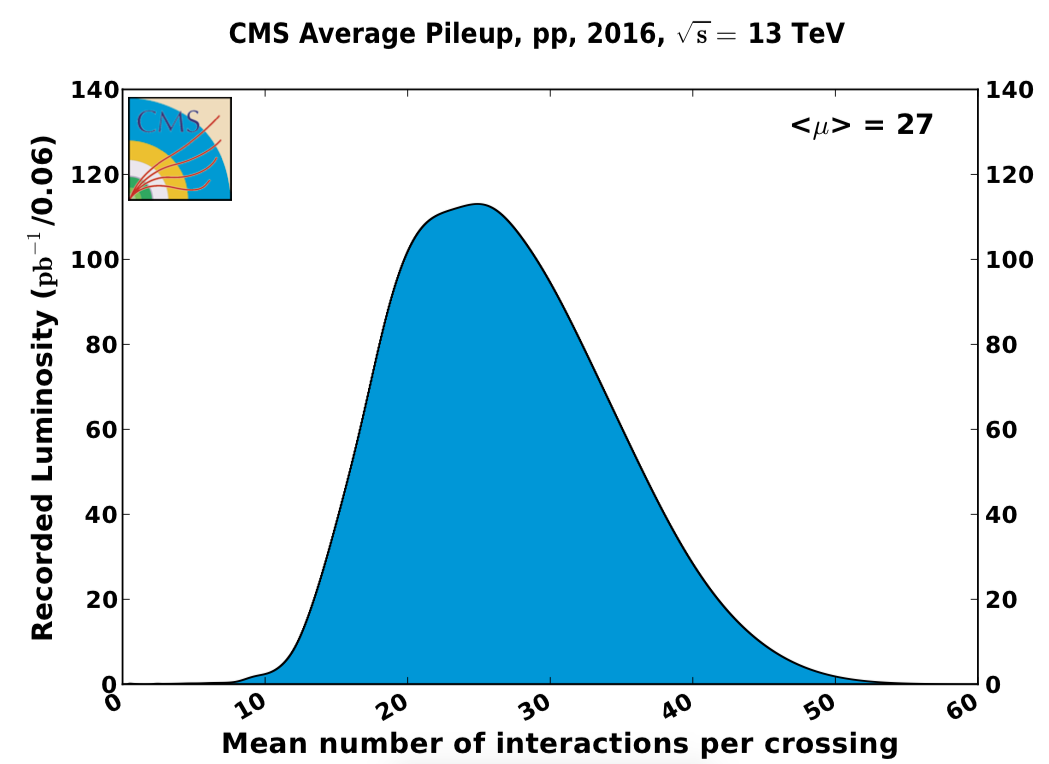
\includegraphics[width=0.72\linewidth]{figures/ob_Nvertex.png}
\caption{Number of interactions per bunch crossing for data collected in 2016.}
\label{fig:ob_Nvertex}
\end{center}
\end{figure}

\subsection{Calorimeter clusters}
The calorimeter clustering serves four purpose in general: detect and measure the energy and direction of stable neutral particles; separate these neutral particles from charged hadron energy deposits; reconstruct and identify electrons and all accompanying bremsstrahlung photons; and help the energy measurement of charged hadrons for which the track parameters were not determined accurately. An algorithm is developed and the clustering process is performed seperately for EB, EE, ES, HB and HE. Firstly cluster seeds are selected as calorimeter cells with deposited energy larger than a threshold and its neighbouring cells. The topological clusters then spread from the seed to the nearby cells with energy beyond cerntain thresholds. Finally a fitting for each topological cluster is performed based on an expectation-maximization algorithm to evaluate position and amplitude of the particle clusters. 

\subsection{Tracks for electrons}
Because of the significant tracker thickness, most of the electrons emit considerable fraction of their energy in the form of bremsstrahlung photons before reaching the ECAL. To reconstruct the properties of an electron, the energy of the bremsstrahlung photons in ECAL must be taken into account as well, apart from the energy deposited by the final electron. A tracker-based electron seeding method was developed. When the radiated energy is small, the electron track can be reconstructed across the whole tracking system with a well-behaved fit $\chi^2$, and the reconstructed momentum should match the energy deposited in the corresponding ECAL cluster. However when energetic photons are radiated, the momentum change of the electron will lead to a large $\chi^2$ and missing hits in the tracker. In these cases, a selection of tracker hits are performed based on the $\chi^2$ value and number of hits in the previous KF fit, and these selected hits are fit again with a Gaussian-sum filter (GSF)~\cite{ob_electronconst} which is more adapted to the electrons as energy losses along the trajectory are considered. 

\subsection{Tracks for muons}
The muons leave their trajectories in the tracking system where the momenta of the muons can be precisely measured, and can be well identified over the full detector especially with the muon chambers. Hits within the DT and CSC detector are clustered to form track segments. These track segments are then used as seeds to reconstruct the muon trajectory throughout DT, CSC, and RPC hits. The result of the final fitting is refered to as a standalone-muon track. With the information of the reconstructed tracks in the tracking system, two collections of high-level muons physics objects can be obtained: the global muon and the tracker muon (See Section~\ref{sec:muonrecon}).

\subsection{Link algorithm}
To reconstruct a physics object, a link algorithm is applied to connect the related PF elements from different subdetectors. The PF elements that can be considered by the algorithem can only be the nearest neighbours in the ($\phi$,$\eta$) plane to any of the elements in the linked block starting from a seed element. The element will be added to the block after the distance of the link is examinated. This process continues until the PF block is formed and the reconstruction of the corresponding particle starts. Links between GSF electron tracks and the ECAL clusters can be established for electrons; links among calorimeter clusters can be established for various particle reconstruction processes, specifically trivial links among ECAL clusters with close $\eta$ but spread $\phi$ form link blocks called superclusters; links between tracks and muon segments can be established for muon reconstruction.

\section{Electron Reconstruction}
The electron reconstruction and identification are performed mainly based on the information from electron tracks in the tracking system and the ECAL clusters. ~\cite{ob_electronconst2}

\vspace{0.3cm}
The electron reconstruction starts from a GSF electron track. In the link algorithm, apart from the electron cluster in ECAL, clusters nearby the extrapolated tangents of the GSF track will also be linked to the PF block as potential bremsstrahlung photons emitted from the electron. A GSF track will be considered a electron candidate if in the PF block the ECAL cluster corresponding to the electron shower is not linked to more than 2 tracks. 

\vspace{0.3cm}
The ECAL clusters in the PF block that can be linked to either the GSF track tangents or the supercluster will be associated with the candidate electron and will be used for the energy calculation of the electron. So is the GSF track if the momentum calculated agrees with the energy deposited in the calorimeters. The position information ($\eta$,$\phi$) assigned to the electron is obtained from the GSF tracks. Once an element is assigned associated to a reconstructed particle, it will be masked against further processing in other object constructions. The calculated energy from the calorimeter clusters will be corrected in terms of energy and $\eta$, to compensate the energy loss in the process. And the final energy assigned to the electron will be obtained from a combination of the corrected energy from the calorimeter clusters and the momentum of the GSF track. 

\vspace{0.3cm}
Furthermore, electrons used in physics analyses must meet additional identification and isolation requirements.

\subsection{Electron Identification and Isolation}
The electron candidates used in this analysis are required to pass the \texttt{loose} cut-based identification (ID) and isolation (Iso) recommended by the CMS EGamma Physics Object Group (POG) for 2016 data.

\vspace{0.3cm}
The ID and Iso criteria set cuts on the following variables, and the cut values are given in Table~\ref{tab:electron-id}.

\begin{itemize}%[noitemsep,nolistsep]
\item the $\eta_{\rm SC}$ denotes the $\eta$ value of the corresponding ECAL super cluster;
\item the $\sigma_{i\eta,i\eta}$ describing the shape of the supercluster;
\item the geometric distance, $|\Delta\eta_{in}|$ and $|\Delta\phi_{in}|$, between the supercluster and the matched track;
\item the ratio of the energy deposits in HCal and ECAL, \texttt{hOverE};
\item the relative combined PF isolation following correction for
  pile-up contamination in the
  Effective Area (EA), \texttt{relIsoWithEA}; % it is the pf Iso used in our analysis 
\item the difference between the tracker momentum and ECAL energy, $|1/E-1/p|$;
\item the maximal expected missing inner hits;
\item a veto on the electrons that are likely to be produced by photon conversions.
\end{itemize}



\begin{table}[htb!]
  \center
  \caption{The cuts used in the POG \texttt{loose} electron identification.}
  \label{tab:electron-id}
  \begin{tabular}{r c c c}
    \hline
    Variable & Barrel & Endcap \\
    \hline
    $|\eta_{\rm SC}|$ acceptance & $(0, 1.479)$ & $(1.479, 2.5)$\\
    $\sigma_{i\eta,i\eta} <$ & 0.011  & 0.0314 \\
    $|\Delta\eta_{in}| <$ & 0.00477  & 0.00868 \\
    $\Delta\phi_{in} <$ & 0.222  & 0.213 \\
    \texttt{hOverE} $<$ & 0.298  & 0.101 \\
    \texttt{relIsoWithEA} $<$ & 0.0994  & 0.107 \\
    $|1/E - 1/p| <$ & 0.241  & 0.14 \\
    expectedMissingInnerHits $\leq$ & 1  & 1 \\
    conversion veto & yes  & yes \\
    \hline
  \end{tabular}
\end{table}

\subsubsection{More About PF Isolation}
The PF isolation requirment is introduced in the electron ID as shown in Table~\ref{tab:electron-id}, in order to suppress the misconstruction rate caused by other particles nearby in the ECAL. The calculation of the PF Iso is based on the PF algorithm: for a given electron or photon, the sum of transverse momenta of all the PF elements with the type of charged hadron, neutral hadron or photon will be calculated if the PF element falls in the isolation cone arround the electron/photon. The cone is usually defined as the region of $\Delta R<0.3$. The separately calculated isolations for the charged hadrons, neutral hadrons and photons can be noted as $Iso_{ch}$,$Iso_{nh}$,$Iso_{photon}$.

\vspace{0.3cm}
Corrections are applied to the calculated PF Iso to compensate the effect caused by contamination from pile-up. In the case of electron Iso, $\rho$-effective area corrections are applied. The effect from the pile-up is considered to be $PU= \rho \times effective_area$, where $\rho$ is the event-specific average pile-up energy density per unit area in the $\phi-\eta$ plane, and the effective area suggests the effective area affected by pile-up for each type of Iso. 

\vspace{0.3cm}
For electrons, the $\rho$-effective area correction does not affect much on the $Iso_{ch}$ term, thus the absolute value of their combined PF isolation is defined in Equation~\ref{eqn:ob_egmiso},
\begin{equation}
Iso=Iso_{ch}+max(0,Iso_{nh}+Iso_{photon}-PU)
\label{eqn:ob_egmiso}
\end{equation}

And the relative isolation shown in Table~\ref{tab:electron-id} is considered to be $relIso=Iso/p_{T}$.

\section{Photon Reconstruction}
The photon reconstruction shares many similarities with electrons, as photons can convert into $e^{-}e^{+}$ pairs and emit bremsstrahlung photons like the electrons. But the reconstruction of photons relies mostly on ECAL. The reconstruction of photon starts from an ECAL supercluster which has no link to a GSF track. The energy deposited in the supercluster will be calculated and ECAL energy correction will also be applied to the supercluster. The result will be assigned to the photon as its energy.

\subsection{Photon Identification and Isolation}
The photon objects used in this analysis are also required to pass the \texttt{loose} cut-based ID and Iso following the recommendation of the EGamma POG. The criteria are listed in Table~\ref{tab:photon-id}.
\begin{table}[htb!]
  \center
  \caption{The cuts used in the POG \texttt{loose} photon identification.}
  \label{tab:photon-id}
  \begin{tabular}{r c c c}
    \hline
    Variable & Barrel & Endcap \\
    \hline
    $|\eta_{\rm SC}|$ acceptance & $(0, 1.479)$ & $(1.479, 2.5)$\\
    $\sigma_{i\eta,i\eta} <$ & 0.0103  & 0.0301 \\
    \texttt{hOverE} $<$ & 0.597  & 0.481 \\
    $Iso_{ch} <$ & 1.295 & 1.011 \\
    $Iso_{nh} <$ & $10.910+0.0148\times p_{T}+0.000017\times {p_{T}}^2$ & $5.931+0.0163*pt+0.000014*pt^2$ \\
    $Iso_{photon} <$ & $3.630+0.0047\times p_{T}$ & $6.641+0.0034\times p_{T}$ \\
    \hline
  \end{tabular}
\end{table}

\vspace{0.3cm}
Unlike electrons, the photon Iso has specific requirements on each type of isolations, instead of a single criterion on a combined Iso value.

\section{Muon Reconstruction}\label{sec:muonrecon}
The CMS muon reconstruction is mainly based on the information collected from the tracker and muon chambers. Generally two collections of muon objects are constructed: the global muon and the tracker muon.~\cite{ob_muonconst}
\begin{itemize}
\item \texttt{Global muon} starts from a stand-alone muon track. If the stand-alone muon track can be matched to a charged-particle track in the tracking system and the properties from the tracks agrees, a globel fit is performed over the two tracks to find a global muon track.
\item \texttt{Tracker muon} starts from a charged-particle track in the tracking system with $p_{T}$ over 0.5 GeV and momentum over 2.5 GeV. If one or more muon segments in the muon chamber system match the extrapolated track of the charged-particle track, then the track is considered a tracker muon track.
\end{itemize}

The reconstruction of global muons and tracker muons are performed separately. A muon can be reconstructed both as a global muon and as a tracker muon and the efficiency of muons reconstructed as either a global muon or a tracker muon is about 99\%.

\vspace{0.3cm}
The momenta calculated from the inner tracks are assigned to the muons with $p_{T}$ less than 200 GeV. For those with $p_T$ beyond 200 GeV, the TuneP algorithm is used: the momenta are calculated from the best fit track among the inner track, the global track, the track combining the inner tracker and the first muon station, and the globally fit track after discarding muon chamber stations with high occupancy. 

\subsection{Muon Identification and Isolation}
Charged hadrons can be faked as muons after reconstruction. To suppress the fake rate of reconstructed muons, identifications are required for muons used in CMS analyses. In this analysis, two types of muon ID are used: the muon \texttt{High $p_T$} ID and \texttt{Tracker High $p_T$} ID. 

\subsubsection{Muon High $p_T$ ID}
The \texttt{High $p_T$} ID is defined below, based on the Muon POG official recommendation for 2016 data analysis.
\begin{itemize}
\item  The candidate is reconstructed as a Global Muon 
\item  At least one muon-chamber hit included in the Global Muon track fit;
\item  Muon segments in at least two muon stations. This implies that the muon is also an arbitrated Tracker Muon; 
\item  The $p_T$ relative error of the muon best track is less than 30\%;
\item  Its tracker track has transverse impact parameter $|dxy| < 2 mm$ with respect to the primary vertex;
\item  The longitudinal distance of the tracker track with respect to the primary vertex is $|dz| < 5 mm$;
\item  At least one pixel hit;
\item  The number of tracker layers with hits is required to be more than 5.
\end{itemize}

The \texttt{High $p_T$} ID is designed aiming at the best reconstruction of the muon track parameters for high-pT muons. To be consistent with the \texttt{High $p_T$} ID, the muon properties obtained from the TuneP algorithm should be used.

\subsubsection{Tracker High $p_T$ ID}
The \texttt{Tracker High $p_T$} ID is a customized muon ID and is modified from the \texttt{High $p_T$} ID, by loosening the global muon requirement to that for a tracker muon, namely removing the following two criteria in the above \texttt{High $p_T$} ID:
\begin{itemize}
\item  The candidate is reconstructed as a Global Muon;
\item  At least one muon-chamber hit included in the Global Muon track fit;
\end{itemize}
and replace them with the following criterion:
\begin{itemize}
\item  The candidate is reconstructed as a Tracker Muon 
\end{itemize}

The \texttt{Tracker High $p_T$} ID is introduced into this analysis to optimize the muon efficiency. The \texttt{Tracker High $p_T$} ID is designed for the identification of a single isolated high $p_T$ muon and would result in decreasing muon efficiency when the muon is from a boosted Z, where the two muons from the Z decay can be too adjacent with each other to be reconstructed as two separated stand-alone muons, in consideration of the limited spatial resolution in the muon detector system. More detail in the efficiency performance can be seen in Section~\ref{sec:muonselection}.

\vspace{0.3cm}
Due to the muon identification choices, in this analysis the muon momentum information used are always obtained from the TuneP algorithm.

\subsubsection{Muon Isolation}
The muons in this analysis are required to be isolated, following the \texttt{loose tracker} isolation recommended by the Muon POG. The sum of the momenta of any charged-particle inner track that does not belong to a muon and appears within the cone of $\Delta R<0.3$ around the muon track is calculated, considered the absolute isolation of the muon and denoted by $Iso_{tk}$. Note that only non-muon tracks are taken into account because our interesting events are characterized by adjacent muon pairs.

\vspace{0.3cm}
The isolation requirment is $relIso_{tk}<0.1$ for each muon selected, where $relIso_{tk}$ is the relative tracker Iso and is defined as $relIso_{tk}=Iso_{tk}/p_{T}$.

\section{Missing Transverse Momentum ($P_T ^{miss}$)}
The Missing Transverse Momentum, denoted by $P_T ^{miss}$ or MET, is calculated as the negative vectorial sum of the momenta of all PF elements~\cite{ob_metconst},
\begin{equation}
\vec{P_T ^miss} = -\Sigma_{i}^{PF} \vec{P_{T,i}}
\label{eqn:ob_metdef}
\end{equation}

It often indicates the existence of undetected particles in the final state of an event, such as neutrinos. But it can also be mismeasured due to the non linearity of the calorimeter response for hadronic particles, tracker inefficiencies and minimum energy thresholds in the calorimeters. This bias can be reduced by applying jet energy corrections~\cite{ob_jetcorr} on the particle level reconstructed jet $P_T$. And thus the corrected missing transverse momentum can be obtained by equation~\ref{eqn:ob_metcorr}, where the superscript "corr" indicates the corrected values.
\begin{equation}
\vec{P_T ^{miss,corr}} = \vec{P_T ^{miss}} - \Sigma_{j}^{jets} (\vec{p_{T,j} ^corr} - \vec{p_{T,j}} )
\label{eqn:ob_metcorr}
\end{equation}

Here the jets are reconstructed on the basis of all types of PF elements, with the Anti-$k_t$ jet clustering algorithm~\cite{ob_jetantikt} with the cone radius $R=0.4$.

